\documentclass{article}
\usepackage{graphicx}
\begin{document}

\section*{Max Flow}

\begin{figure}
\begin{center}
 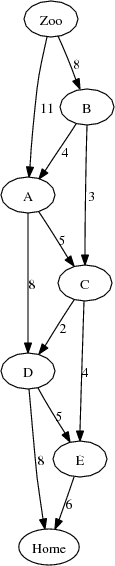
\includegraphics[width=150pt,height=500pt]{MaxFlow.png}
 % NetworkFlow2.pdf: 612x792 pixel, 72dpi, 21.59x27.94 cm, bb=0 0 612 792
\end{center}
\caption{A map of the public transportation network from the zoo to Home}
\end{figure} 

A panda is about to give birth at the zoo!  Officials anticipate that attendance will skyrocket to see the new, adorable baby panda.  There's one particular residential area called ``Home'' that is full of panda loving families and there's a fear that this inflated number of people visiting the zoo will overload the public transportation system.  It will be especially bad in the evening since the zoo closes about the same time as rush hour, so everyone will be trying to find spaced on the already crowded buses and subways.  As a city planner, you were given a map of routes from the zoo to Home (shown below), along with the estimated number of families that could go on each route.  Additionally, it was estimated that $16$ families from Home will visit each day, and it's your task to figure out if this will overload the public transportation system, and, if it does, how could the system be improved?

This is another kind of network flow problem, called a maximum flow problem.  Here, what we're concerned about is the upper bound on the amount of people that can move through the system.  This is a special case of network flow problems, but it's also one of the most relevent and easily applicable kinds of problems.  Unlike previous examples, we're not trying to minimize cost; instead we're trying to find the maximum amount of flow, which is defined by the number of objects moving thrugh the system.  In this case, our flow is how many people can travel from the zoo to Home.

Before we begin the implementation, it's worth briefly covering some key points of a network.  Typically, the locations we're looking at are called ``nodes'' and the paths between them are ``arcs,'' which should be familiar to anyone who has with graph theory.  Additionally, nodes that have an excess supply are called ``sources'' while nodes with an excess of demand are ``sinks.''  All other nodes should have a net change of zero---anything that flows in should also flow out.  In this example, our source is the zoo and our sink is Home, while all the locations between the two should not supply any people and no people should stop at them.

With this, we can now construct a model.

\subsection*{Build the model}

As always, start by importing Pyomo and creating an object of the class model.

\begin{verbatim}
from pyomo.core import *

model = AbstractModel()
\end{verbatim}

Now, we must define our sets.  The set of locations, which we'll call nodes, is fairly typical.  Additionally, we must create a set of arcs.  Since each arc is a tuple from the set of nodes crossed with itself, we must define it slightly differently.  This is very similar to how we defined the routes in the first network flow problem---in fact, the only difference is the names of the sets.

\begin{verbatim}
model.nodes = Set()
model.arcs = Set(within=model.nodes*model.nodes)
\end{verbatim}

The ``within='' notation implies that we're creating a subset of something else---in this case arcs is a subset of all the tuples that could be generated by the nodes crossed with themselves.  This is important since the set of sources and sinks are going to be defined as subsets of the set of nodes.  In code, this looks like:

\begin{verbatim}
model.sources = Set(within=model.nodes)
model.sinks = Set(within=model.nodes)
\end{verbatim}

\noindent
While we only have one source and sink in this example, it's often useful to create a more general model than necessary.  This same model can be used next week to find the maximum flow between three office building and four residential areas, for example.

We now consider the parameters.  Each arc has an upper bound on how many families can travel along it, so we create a parameter over the set of arcs.

\begin{verbatim}
model.upperBound = Param(model.arcs)
\end{verbatim}

We will also create a supply parameter over the set of sources and a demand parameter for the sinks.  Since we're just looking for the max supply in this problem, the supply parameter will be arbitrarily large and the demand parameter will be $0$ when we define them in the data file.  This way, the program won't accidentally crash with an infeasible model and we can guarantee we achieve the max flow.  However, in other cases it might be useful to have an explicit number for the supply at each source or demand at each sink, so we include it to make the model more general.

\begin{verbatim}
model.supply = Param(model.sources)
model.demand = Param(model.sinks)
\end{verbatim}

Finally, we need to define a variable.  Like the previous examples, this variable will be the amount that goes along each arc; in this case it will be how many families travel on each path between the zoo and Home.  As usual, we restrict the domain to non negative numbers since, simply put, negative families don't make sense.  

\begin{verbatim}
model.amount = Var(model.arcs, within=NonNegativeReals)
\end{verbatim}

At this point, we must now begin constructing the objective and constraints.  The objective of this problem is to maximize the number of people flowing into Home, which is a very different objective than what we've done before; unlike the previous cases, we're not trying to minimize a value.  Additionally, in previous examples we would just take the dot product of the cost and amount vectors, which isn't helpful in this case.

Solving these two problems is pretty simple, fortunately.  To begin with, to maximize the objective we just insert ``sense=maximize'' into the arguments the objective takes, which will tell the model to try and maximize this value.  Similarly, we could have put ``sense=minimize'' in the previous examples, but since the objective naturally tries to minimize the rule it takes in, this would be redundant.

The other problem we ran into was how to measure the number of people who arrive at Home.  The most logical way to do this is take every arc that ends at home, find the amount of people traveling along it, and sum those values together.  For the code, though, we're being a bit more general since in this abstract model there could be multiple sinks (rather than just Home).  The logic is still the same: just find the amount traveling on each arc that goes into a sink and add those values together.

\begin{verbatim}
def totalRule(model):
    expression = sum(
      model.amount[i,j]
      for (i, j) in model.arcs
      if j in model.sinks
    )
    return expression

model.maxFlow = Objective(rule=totalRule, sense=maximize)
\end{verbatim}

Another important element of this model is the maximum amount that can travel on each route.  Without that, the max flow problem would be trivial: the answer is always infinity!  To avoid this situation, we need to ensure that the amount traveling along each arc is less than or equal to the upper bound of how much can move along the arc.  One part that deserves note is that we give the constraint the set of arcs as an argument, but in defining the rule we give it two arguements: arcIn and arcOut.  The reason for this is because the set of arcs is itself a set of tuples, so when we feed it in as an argument we're actually supplying two arguements.  The final result will be this:

\begin{verbatim}
 def maxRule(arcIn, arcOut, model):
    constraint_equation = (model.amount[arcIn, arcOut] 
      <= model.upperBound[arcIn, arcOut])
    return constraint_equation

model.loadOnArc = Constraint(model.arcs, rule=maxRule)
\end{verbatim}

We have one last rule to consider: the flow rule.  The idea behind the flow rule is that something traveling along the network won't just appear or disappear.  The amount that flows into a location must be equal to the amount that flows out, with the exception of sinks and sources.  It's this last part that makes the constraint complicated since we now have three cases---the node is regular, a source or a sink---that must each be treated slightly differently.

What we will do is define a flow rule that takes in a node as an argument, then use ``if...then...else'' statements to look at all possible cases.  In each case we'll create a value called ``constraint\_equation'' and at the end the flow rule will return the constraint\_equation.  As a rough outline of what the code will look like, we have

\begin{verbatim}
def flowRule(node, model):
    if node in model.sources:
      ...
      constraint_equation =...
    
    elif node in model.sinks:
        ...
        constraint_equation = ...
    else:
        ...
        constraint_equation = ...
    
    return constraint_equation

model.flow = Constraint(model.nodes, rule=flowRule)
\end{verbatim}


We begin with the case where the node is a source, we want to ensure that the flow out is less than or equal to the supply of the node.  To find flow out of a source, we just find every arc that begins at the source and sum the amounts on them together, must like we did when defining the objective earlier.  We then just need to make sure that the flow out of each arc will be less than its supply.  In code, this will look like

\begin{verbatim}
 if node in model.sources:
      flow_out = sum(
        model.amount[i,j] 
        for (i,j) in model.arcs 
        if i == node
      )
      constraint_equation = (flow_out <= model.supply[node])
\end{verbatim}

In the next case we look at, the node is a sink.  This is structured almost identically to the previous case, the main difference being we're looking at where the arcs end rather than begin, and we need to be greater than or equal to demand.

\begin{verbatim}
 elif node in model.sinks:
      flow_in = sum(
        model.amount[i,j]
        for (i,j) in model.arcs
        if j == node
      )
      constraint_equation = (flow_in >= model.demand[node])
\end{verbatim}

Finally, we have the case where the node is ``normal.''  Here, we need to ensure that the amount flowing in is equal to the amount flowing out.  This is much like the previous two cases combined: we create an ``amountIn'' value that adds up the amount on each arc ending in the node, and we create an ``amountOut'' value that adds the amount on each arc that originates at the node.  We then create a constraint equation to ensure that amountIn and amountOut are equal.

\begin{verbatim}
 else:
      amountIn = sum(
        model.amount[i,j] 
        for (i,j) in model.arcs 
        if j == node
      )
      amountOut = sum(
        model.amount[i,j] 
        for (i,j) in model.arcs 
        if i == node
      )
      constraint_equation = (amountIn == amountOut)
\end{verbatim}

Putting these three cases together, along with the outline we had before, yields the constraint we wanted.

\begin{verbatim}
def flowRule(node, model):
    if node in model.sources:
        flow_out = sum(
          model.amount[i,j] 
          for (i,j) in model.arcs 
          if i == node
        )
        constraint_equation = (flow_out <= model.supply[node])
    
    elif node in model.sinks:
        flow_in = sum(
          model.amount[i,j]
          for (i,j) in model.arcs
          if j == node
        )
        constraint_equation = (flow_in >= model.demand[node])
    
    else:
        amountIn = sum(
          model.amount[i,j] 
          for (i,j) in model.arcs 
          if j == node
        )
        amountOut = sum(
          model.amount[i,j] 
          for (i,j) in model.arcs 
          if i == node
        )
        constraint_equation = (amountIn == amountOut)
        
    return constraint_equation
    
model.flow = Constraint(model.nodes, rule=flowRule)
\end{verbatim}

Save this model as a .py file before continuing.

\subsection*{Data entry}

The data entry for this problem is fairly routine after the previous examples.  We begin by defining our sets.  Remember, arcs is a subset of nodes crossed with itself and sources and sinsk are subsets of nodes.  This just means you can't input arbitrary values---they have to be values from the proper sets.

\begin{verbatim}
set nodes := Zoo A B C D E Home;
set arcs := (Zoo,A) (Zoo,B) (A,C) (A,D) (B,A) (B,C) (C,D) (C,E) 
            (D,E) (D,Home) (E,Home);
set sources := Zoo;
set sinks := Home;
\end{verbatim}

We also need to define the supply and demand parameters.  These are especially easy because the sets they're over only have one element.  Remember, for this example the supply is abitrarily large and demand is zero so we won't accidentally create an infeasible model.

\begin{verbatim}
param: supply :=
Zoo 1000000;

param: demand :=
Home 0;
\end{verbatim}

Finally, we create the upper bound parameter.  This, is a paramater over tuples, but we must omit the parentheses and commas that usually denote such a tuple.  Otherwise, it's formated the same way as the above parameters.

\begin{verbatim}
param: upperBound :=
Zoo A 11
Zoo B 8
A C 5
A D 8
B A 4
B C 3
C D 2
C E 4
D E 5
D Home 8
E Home 6;
\end{verbatim}

Now, save this file as a .dat file.

\subsection*{Solution}

For a Linux machine, go to the command line and input ``pyomo [model].py [model].dat'' where [model] is replaced with what you named the file.  If using the files from the Pyomo directory, it would be ``pyomo maxFlow.py maxFlow.dat''

\begin{verbatim}
# ==========================================================
# = Solver Results                                         =
# ==========================================================

# ----------------------------------------------------------
#   Problem Information
# ----------------------------------------------------------
Problem: 
- Lower bound: -inf
  Upper bound: 14
  Number of objectives: 1
  Number of constraints: 18
  Number of variables: 12
  Number of nonzeros: 32
  Sense: maximize

# ----------------------------------------------------------
#   Solver Information
# ----------------------------------------------------------
Solver: 
- Status: ok
  Termination condition: unknown
  Error rc: 0

# ----------------------------------------------------------
#   Solution Information
# ----------------------------------------------------------
Solution: 
- number of solutions: 1
  number of solutions displayed: 1
- Gap: 0.0
  Status: optimal
  Objective: 
    f: 
      Id: 0
      Value: 14
  Variable: 
    amount[D,Home]: 
      Id: 0
      Value: 8
    amount[E,Home]: 
      Id: 1
      Value: 6
    amount[B,C]: 
      Id: 2
      Value: 3
    amount[B,A]: 
      Id: 3
      Value: 4
    amount[Zoo,B]: 
      Id: 4
      Value: 7
    amount[Zoo,A]: 
      Id: 5
      Value: 7
    amount[D,E]: 
      Id: 6
      Value: 2
    amount[A,C]: 
      Id: 7
      Value: 3
    amount[A,D]: 
      Id: 8
      Value: 8
    amount[C,D]: 
      Id: 9
      Value: 2
    amount[C,E]: 
      Id: 10
      Value: 4

\end{verbatim}

This output tells us how many people should travel along each route for the optimal solution.  More importantly, though, is the line which says our objective value is $14$.  This means that at most $14$ families can arrive at Home.  However, we were told $16$ families from Home were expected to visit the zoo each day.  Therefore, unless something is done, the public transportation network in place will be overloaded.

In looking at the data, your bosses noticed that not many people can travel the route from C to D; it only has room for $2$ more families.  It's decided to add more buses to that route, and after new calculations are done it's believed that up to $12$ families will be able to travel that route!  Your bosses believe they've solved the problem, but you're not so sure.  Let's double check the results to see what happens.

Change the upper bound information on the arc from C to D so it carries $12$ people rather than $2$ and run Pyomo again.  The result is...pretty much the same.  While the amount on each path might be different, the overall max flow is still the same.  Why is that?

Only two paths lead to Home, one beginning at D and one beginning at E.  The former path can hold up to $8$ families and the latter can hold $6$.  This means, at most $8+6=14$ families will be able to travel into Home.  So to solve this problem it's not enough to boost the amount of people who travel from C to D, but also from D to Home (or E to Home).  We change the upper bound of the route from D to Home to $10$ and run the model again.  This time our max flow is $16$!  Note, though, that if the bound on the arc from C to D is still $2$ then the max flow is still only $14$.  

We can now present our results, recommending what needs to be changed---increasing the number of buses on the C to D and D to Home routes---in order to boost the max flow through the public transportation network to $16$ families to accommodate the families traveling to the zoo to see the adorable panda baby.

\end{document}
